\documentclass[a4paper,10pt,titlepage]{report}
%%This template is based on Paco van Beckhoven's thesis. 

\usepackage{xspace}
\usepackage{xargs}   % Use more than one optional parameter in a new commands
\usepackage[pdftex,dvipsnames]{xcolor}

% Putting images next to each other
\usepackage[font=bf,]{caption}
\usepackage{subcaption}
\input{glyphtounicode}

% for last page
\usepackage{lastpage}

\usepackage[english]{babel}
\usepackage[utf8]{inputenc}
\usepackage{csquotes}
\usepackage[margin=1in]{geometry}
\usepackage{fancyhdr}
\usepackage{booktabs}
\usepackage{paralist}
\usepackage{graphicx}
\usepackage{tabularx}
\usepackage{adjustbox}
\usepackage{titlepic}
\usepackage{vhistory}
\usepackage{enumitem}
\usepackage{longtable}
\usepackage[backend=biber, style=ieee,citestyle=numeric-comp]{biblatex}
\usepackage[colorinlistoftodos, prependcaption]{todonotes}
\usepackage{placeins}
\usepackage{multirow}
\usepackage{amsmath,amssymb}
\usepackage[hidelinks]{hyperref}
\usepackage[acronym,nogroupskip,nohypertypes={acronym},toc,section=chapter]{glossaries}
\usepackage{amssymb}
\usepackage{verbatim}
\usepackage{cmap}
\usepackage{float}

%\usepackage[ansinew]{inputenc}
%\usepackage[T1]{fontenc}
%\usepackage{libertine}
\input{glyphtounicode}

\pdfglyphtounicode{f_f}{FB00}
\pdfglyphtounicode{f_f_i}{FB03}
\pdfglyphtounicode{f_f_l}{FB04}
\pdfglyphtounicode{f_i}{FB01}

\pdfgentounicode=1



%Appendix package + appendix in chapter title
\usepackage[titletoc]{appendix}




%for highlighting findings
\usepackage{tcolorbox}

% for highlighting code examples
\usepackage{listings}

\newcommand{\ie}{\emph{i.e.},\xspace}
\newcommand{\eg}{\emph{e.g.},\xspace}
\newcommand{\etc}{\emph{etc.}\xspace}
\newcommand{\etal}{\emph{et al.}\xspace}

\newcommand{\sig}{\gls{sig}}
\newcommand{\sigs}{\glspl{sig}}

\newcommandx{\unsure}[2][1=]{\todo[linecolor=red,backgroundcolor=red!25,bordercolor=red,#1, inline]{#2}}
\newcommandx{\discussion}[2][1=]{\todo[linecolor=red,backgroundcolor=green!25,bordercolor=red,inline,#1]{#2}}

\newcommandx{\improvement}[2][1=]{\todo[linecolor=blue,backgroundcolor=blue!25,bordercolor=blue,#1]{#2}}

\newcommandx{\reminder}[2][1=]{\todo[linecolor=yellow,backgroundcolor=yellow!25,bordercolor=yellow,#1]{#2}}

\newcommandx{\lessprio}[2][1=]{\todo[linecolor=Plum,backgroundcolor=Plum!25,bordercolor=Plum,#1]{#2}}
\newcommandx{\todocontent}[2][1=]{\todo[author=\textbf{Planned content},backgroundcolor=Goldenrod!25,bordercolor=Goldenrod,inline,#1]{#2}}


%%Some additional table column specifiers, allowing for fixed width columns that wrap.
\newcolumntype{L}[1]{>{\raggedright\let\newline\\\arraybackslash\hspace{0pt}}p{#1}}
\newcolumntype{C}[1]{>{\centering\let\newline\\\arraybackslash\hspace{0pt}}p{#1}}
\newcolumntype{R}[1]{>{\raggedleft\let\newline\\\arraybackslash\hspace{0pt}}p{#1}}

\definecolor{ryel}{HTML}{fcd116}
\definecolor{rred}{HTML}{ce1126}
\definecolor{rblu}{HTML}{0a3eb9}
%these are examples of commands that may facilitate feedback annotations in the document
%replace \paco by your name and \ana by your supervisor's name
%\newcommandx{\ana}[2][1=]{\todo[linecolor=rblu,backgroundcolor=ryel,bordercolor=rred,#1]{#2}}
%\newcommandx{\paco}[2][1=]{\todo[author=Paco,linecolor=blue,backgroundcolor=white,bordercolor=red,#1]{#2}}


% -- title page is a modified version of https://github.com/software-engineering-amsterdam/latex/blob/master/thesis/uvamscse.cls
\newcommand{\email}[1]{\ttfamily\href{mailto:#1}{#1}}

\newcommand{\uvacoverfoot}{%
	\vfill
	\begin{center}
		\begin{tabular}{r|l}
			\multirow{3}{*}{
\includegraphics[height=48pt]{uva.pdf}}
			&\textsc{\Large University of Amsterdam}\\
			% &\textsc{Faculteit der Natuurwetenschappen, Wiskunde en Informatica}\\
			&\textsc{Master Security and Network Engineering}\\
			&\url{http://www.os3.nl/}
		\end{tabular}
	\end{center}
}

\renewcommand{\maketitle}{%
	% The cover page
	% --------------
	\thispagestyle{empty}
	\enlargethispage{30pt}
	\renewcommand{\thefootnote}{\fnsymbol{footnote}}
	% Will be page 0, s.t. contents start on page 1
	\setcounter{page}{0}
	% \eccoverhead
	% Volume and article title, author(s)
	\vspace{60pt}
	\begin{center}
		{\Huge\bfseries Feature Selection on a Differentially Private Dataset \par}
		\vspace{11pt}
        { Short project (1 month) \par}

        
		\vspace{11pt}
        {\Large Project proposal \par}
		
		\vspace{44pt}
		{\Large\bfseries Nick Moone \par}
		\email{nick.moone@os3.nl}\\
		\vspace{11pt}
		\today, \pageref{LastPage} pages
	\end{center}
	\vfill
    \begin{center}
    	\begin{tabular}{ll}
    		\textbf{Academic supervisor:} 	& Mina Alishahi, \email{mina.sheikhalishahi@ou.nl} \\
    		\textbf{Supervisor affiliation:} & Open Universiteit, \url{https://www.ou.nl/}
    	\end{tabular}
    \end{center}
	\uvacoverfoot
	\newpage
	\setcounter{footnote}{0}
	\renewcommand{\thefootnote}{\arabic{footnote}}
	\setlength{\parskip}{0pt}
}

%\newcommand{\uvaabstract}{}latex 
%\renewcommand{\abstract}[2][Abstract]{\renewcommand{\uvaabstract}{\chapter*{Abstract}%
%\par#2\newpage}}


%-------- End of ``title page''

%Fancy page headers
\pagestyle{fancy}
\fancyhf{}
\fancyhead[L]{\leftmark}
\fancyfoot[C]{\thepage}
\setlength{\headheight}{14pt}


%%FINDING ENV
\newcounter{findingctr}

\newenvironment{finding}{%      define a custom environment
	\refstepcounter{findingctr}% increment the environment's counter
	\begin{tcolorbox}
	\textbf{Finding \thefindingctr:}
}{\end{tcolorbox}} 
% If you want numbers that start with the chapter or section number (e.g. 7.1.1 or 7.1) enable the following lines 
%\usepackage{amsmath}
%\numberwithin{findingctr}{chapter}


% Decrease the size of all these lists
\setlist{noitemsep,topsep=4pt,parsep=1pt,partopsep=4pt}


\lstset{
	basicstyle=\footnotesize,        % the size of the fonts that are used for the code
	breakatwhitespace=false,         % sets if automatic breaks should only happen at whitespace
	breaklines=true,                 % sets automatic line breaking
	captionpos=b,                    % sets the caption-position to bottom
	frame=single,                    % adds a frame around the code
	language=Java,                 % the language of the code
	keywordstyle=\bf,
	tabsize=2                       % sets default tabsize to 2 spaces
}

%make it fit more nicely
\setlength\extrarowheight{2pt}


%helpful acronym examples
\newacronym{cc}{CC}{Cyclomatic Complexity}

\newacronym{sut}{SUT}{System Under Test}

\newacronym{strew}{STREW}{Software Testing and Reliability Early Warning}

\newacronym{sig}{SIG}{Software Improvement Group}

\newacronym{sat}{SAT}{Software Analysis Toolkit}

\newacronym{tloc}{TLOC}{Lines Of Test Code}
\newacronym{loc}{LOC}{Lines of Code}

\newacronym{taime}{TAIME}{Test Suite Assessment and Improvement Method}

\newacronym{tqm}{TQM}{Test Quality Model}

\newacronym{tdd}{TDD}{Test-Driven Development}

\newacronym{cor}{COR}{Conditional Operator Replacement}
\newacronym{ror}{ROR}{Relational Operator Replacement}
\newacronym{ast}{AST}{Abstract Syntax Tree}
\makeglossaries
\bibliography{main}

\begin{document}



\maketitle
\begin{abstract}
    Privacy concerns have become increasingly prominent in data analysis, leading to adoption of privacy-preserving approaches such as the use of differentially private synthetic data. However, these approaches may impact the significance of features in the synthetic dataset, potentially affecting the accuracy and reliability of subsequent machine learning tasks. Previous research explored the preservation of feature significance in a dataset after anonymization techniques were applied. As anonymization techniques cannot entirely prevent re-identification of individuals in datasets, this research builds upon the earlier work by investigating the impact of applying differential privacy techniques on feature significance.
\end{abstract}
% \tableofcontents
\chapter{Introduction}
\label{ch:introduction}
In the age of data-driven decision-making and machine learning applications, safeguarding data privacy has emerged as a critical concern. With the use of personal data for these applications, methods are required for anonymizing data to protect the origin's identity. Privacy preserving and anonymization techniques exist, but these approaches may impact the significance of features in the original dataset, potentially affecting the accuracy and reliability of subsequent machine learning tasks. Previous research explored the preservation of feature significance in a dataset after anonymization techniques were applied \cite{originalpaper}. As anonymization techniques cannot entirely prevent re-identification of individuals in datasets \cite{dpuitleg}, this research builds upon the earlier work by investigating feature selection after applying differential privacy techniques as a stronger privacy mechanism.

Feature significance allows for understanding the relationships between the features and the target variables in a dataset, which plays a crucial role in data analysis and machine learning tasks. Its primary motivation stems from the desire to enhance model performance, reduce computation costs, and mitigate the risk of overfitting. By selecting the most relevant and informative features from a potentially large and noisy dataset, the efficiency and accuracy of models can be improved. The preservation of feature significance gives an indication of how well the dataset after making it differentially private is suitable for data analysis and machine learning tasks.

Transforming a dataset into a differentially private dataset may influence the datasets' features' significance, potentially making it less suitable for data analysis and machine learning. Differential privacy techniques add a provable privacy guarantee to individuals in an original dataset, and at the same time it attempts to maintain properties (e.g., schema and correlations between attributes) of the original dataset \cite{dpuitleg}. This research will explore till what extend the features' significance of a dataset is influenced by applying differential privacy techniques on it.

By ensuring that the significance of features is retained during anonymization processes, we can protect the performance and interpretability of machine learning models, enabling them to make more accurate predictions at less costs.\\

Our research presents a comprehensive investigation of the implications of applying differential privacy techniques implemented by the PrivSyn algorithm \cite{privsyn} on feature's significance, it is driven by the need to explore the trade-offs between privacy preservation and data utility. We answer five fundamental research questions that explore various dimensions of feature significance in the context of differential privacy. By doing this we aim to provide insights into the effects of making a dataset differentially private using various differential privacy parameters on the interpretability, accuracy, and generalizability of classifiers trained on differentially private datasets.

% TODO laatste deel van intro mina paper met contributions

% TODO problem statement uit paper (architecture figure en uitleggen waarom dit nodig is)

\section{Research questions}
We guide our research using the following research questions:\\
\textbf{RQ1} Which feature selection technique outperforms the others in preserving the significant scores of features in a dataset?
Here we evaluate the performance of various feature selection techniques on the preservation of features' significance in differentially private datasets compared to the original datasets. We do this by employing four widely recognized filter-based feature selection methods. With this analysis we aim to identify the feature selection technique that best retains the characteristics of the original datasets in the differential private datasets, so we can use this feature selection technique to answer our further research questions.

\textbf{RQ2} How do the correlation patterns between features change in the differentially private dataset compared to the original one?
Here we explore how the correlation patterns between features change when transforming a dataset into a differentially private dataset. To do this we compute the correlation matrices for both the original and the differentially private dataset. Comparing these gives us a measure of how strongly correlated features are related in a dataset, and how making the dataset differentially private affects strongly correlated features.

\textbf{RQ3} How does the variation in input datasets’ properties, such as dataset size, number of features, and number of labels, influence the preservation of features’ importance?
Here by investigating the impact of input dataset characteristics, we aim to gain insight into the relationship between dataset properties and the ability to maintain the significance of features in the differentially private dataset.

\textbf{RQ4} How does the variation of differential privacy techniques’ parameters impact the preservation of features’ importance?
Here we explore the effects of adjusting the privacy parameters of the differential privacy algorithm on the significance of features. With this question we aim to find a balance between privacy protection and data utility.

\textbf{RQ5} How does feature selection, specifically the removal of irrelevant features, impact the accuracy of classifiers trained on both the original and differentially private datasets?
With this research question we investigate the effect of feature selection on a differentially private dataset. We do this by comparing the performance of classifiers trained on selected features of both the original dataset and the differentially private dataset.

% TODO
% \section{Contributions}
% Our research makes the following contributions:
% \begin{enumerate}
% 	\item 
% 	\item An analysis of the impact of transforming a dataset into a differentially private dataset on its feature significance.
% 	\item An analysis the impact of the impact of datasets' properties, e.g., dataset size, in preserving the features' importance.
% \end{enumerate}

\section{Ethical considerations}
This research was done in an ethical way, adhering to ECOS3 \cite{ecos3} procedures. This means that the ECOS3 responsible disclosure procedure was followed, and we planned to immediately contact ECOS3 upon encountering unforeseen ethical circumstances to discuss how to continue our research.

All datasets used for this research are from the public datasets as a service repository of UCI \cite{datasetsrepo}, all datasets in this repository are non-sensitive and allow the use by anyone. Other than these datasets no data will be used for this research.

The project aims at improving privacy when sharing data for machine learning purposes. We expect that no malicious activities can be performed as a result of publishing our findings.

% \section{Project scope}

% \section{Outline}
% In Chapter~\ref{ch:background} we describe the background of this thesis. 
% Chapter~\ref{ch:research} describes ... 
% Results are shown in Chapter~\ref{ch:results} and discussed in Chapter~\ref{ch:discussion}. Chapter~\ref{ch:related_work}, contains the work related to this thesis.
% Finally, we present our concluding remarks in Chapter~\ref{ch:conclusion} together with future work.


% \chapter{Background}
\label{ch:background}

\section{Feature selection}
Feature selection highlights the significance of features in a dataset \cite{featureselectionzhang}, it is a technique for optimizing datasets and allows for efficient data analysis and machine learning tasks. The main motivations for feature selection are enhancing the models' performance, reducing computation cost, and mitigating the risk of overfitting.
By selecting only the most relevant and informative features from a large and noisy dataset, the size of the dataset can be reduced while maintaining its feature significance. Resulting in simpler, better interpretable, and more robust models.

\subsection{Feature selection methods}
Four well-known feature selection methods are considered: Chi-square, Information Gain, Anova F-Value, and Pearson correlation. These methods calculate significance scores for each individual feature in a dataset, allowing for the ranking of features based on their significance.
\paragraph{Chi-square}
($\chi^2$) is typically used in statistics to test the independence of two events. In feature selection, the $\chi^2$ test is used to test whether the occurrence of a specific feature $A_k$ and class labels $C$ are independent \cite{originalpaper}.

Its score is calculated using the following formula:
\begin{align}
    \mathcal{J}_{\chi^2}(C,A_k) = \sum_{l=1}^{L}\sum_{j=1}^{|A_{k}|}\frac{n_{0}(c_{l},v^{k}_{j}) - n_{e}(c_{l},v^{k}_{j})}{n_{e}(c_{l},v^{k}_{j})},
\end{align}
where $n_{0}(c_{l},v^{k}_{j}$ is the number of instances with class label $c_l$ and respecting the $j$'th value of feature $A_k$; and
\begin{align}
    n_{e}(c_{l},v^{k}_{j}) = \frac{n_{0}(c_{l})*n_{0}(v^{k}_{j})}{n},
\end{align}
where $n$ is the total number of records in the dataset, and $n_{0}(c_{l})$ and $n_{0}(v^{k}_{j})$ are the number of records with class label $c_l$ and the ones with value $v^{k}_{j}$ respectively. The higher value of $\mathcal{J}_{\chi^2}(C,A_k)$ shows a higher dependency between the feature and class labels.

\paragraph{Information Gain}
gives a measure of the amount of shared information between a feature and class labels in a dataset \cite{originalpaper}. Let $A_k$ and $C$ be two discrete variables, the entropy of $C$ is defined as:
\begin{align}
    H(C) = -\sum_{c_l \in C}{p(c_l)log_{2}(p(c_l))},
\end{align}
where $p(c_l)$ is the probability of $c_l$ occurring in the dataset. The conditional entropy of $C$ given $A_k$ is computed as:
\begin{align}
    H(C|A_k) = -\sum_{v^{k}_{j} \in A_{k}} \sum_{c_{l} \in C} p(v^{k}_{j})p(c_{l}|v^{k}_{j}) log_{2}(p(c_{l}|v^{k}_{j})).
\end{align}
The information gain of variable $A_k$ dependent to variable $C$, the mutual information of $A_k$ and $C$, is defined as:
\begin{align}
    \mathcal{I}(C, A_{k}) = H(C) - H(C|A_k)
\end{align}
The higher value of $\mathcal{I}(C, A_{k})$ shows more relevance of the feature in class discrimination.

\paragraph{Anova F-value}
determines the ratio of explained variance to unexplained variance \cite{originalpaper}. In the context of feature selection, for each feature the hypotheses are defined as:\\

$H_{0} : \mu_{1} = \mu_{2} = ... = \mu_{L}$, $H_{1} : \mu_{1}, \mu_{2}, ..., \mu_{L}$ are not equal,\\

where $\mu_{l}$ is the mean of the $l$'th class. The total mean is computed as $\mu = \frac{1}{n} \sum^{L}_{l=1} n_{l} \mu_{l}$ for $n_l$ being the number of records respecting class label $c_l$. The mean of samples for feature $A_k$ is computed as $\overline{x^k} = \frac{1}{n} \sum^{n_k}_{j=1}x_{ij}$, while the total average $\overline{x}$ is computed as $\overline{x} = \frac{1}{n} \sum^{L}_{l=1} \sum^{n_k}_{i=1} x_{il}$. Accordingly, the sum of mean squared within groups ($S_E$) and the sum of mean squared deviation between groups ($S_A$) are computed as:
\begin{align}
    S_{E} = \sum^{L}_{l=1} \sum^{n_k}_{i=1} (x_{il} - \overline{x_{k}})^2, S_{A} = \sum^{L}_{l=1} \sum^{n_k}_{i=1} (\overline{x_{k}} - \overline{x})^2.
\end{align}
Then, the Anova F-value is computed as $F = \frac{S_{A}/(L-1)}{S_{E}/(n-L)}$. The higher value of $F$ shows a higher correlation between a feature and the class labels.

\paragraph{Pearson correlation coefficient} is a statistical measure quantifying the linear relationship between two variables \cite{originalpaper}. The Pearson correlation coefficient ($r$) between feature $A_k$ and class $C$ is calculated as:
\begin{align}
r(C, A_{k}) = \frac{\sum^{n}_{i=1}(x^{k}_{i} - \overline{x^{k}}) (x^{C}_{i}-\overline{x^{C}})}{\sqrt{\sum^{n}_{i=1}(x^{k}_{i}-\overline{x^{k}})^{2} \sum^{n}_{i=1}(x^{C}_{i}-\overline{x^{C}})^2}},
\end{align}
where $n$ is the number of records in the dataset, $x^{k}_{i}$ and $x^{C}_{i}$ represent the values of feature $A_k$ and class $C$ for the $i$th data point, $\overline{x^{k}}$ and $\overline{x^{C}}$ are the means of feature $A_k$ and class $C$ respectively. The Pearson correlation coefficient ranges from -1 to 1, where a value of 1 indicates a perfect positive linear correlation between a feature and the class; a value of -1 indicates a perfect negative linear correlation between a feature and the class; and a value of 0 indicates no linear relation between the feature and the class.
A high absolute value of the Pearson correlation coefficient between a feature and the class indicates a strong correlation.

\section{Differential privacy}
Differential privacy techniques are techniques for transforming a dataset into a synthetic dataset. It is an improvement over various anonymization techniques because the synthetic differentially private dataset has the original schema, it aims at maintaining correlation patterns, and it provides a provable privacy guarantee for the individuals in the original dataset \cite{dpuitleg}.

A downside of differential privacy is that the data in the resulting synthetic dataset is a less accurate representation of the original data than most anonymization techniques provide \cite{dpuitleg}, but many use cases do not require the most accurate representations.

\subsection{Differential privacy parameters}
\label{sec:difprivparams}
Differential privacy uses two parameters that need to be considered for applying it, $\delta$ and $\epsilon$. Both parameters indicate how much privacy is desired in the resulting synthetic dataset. 

$\delta$ represents chance that someones privacy is compromised when the data is accidentally being leaked \cite{dpparams}, lower values of $\delta$ provide higher privacy and more noise added to the data. The value of $\delta$ is usually fixed to $\frac{1}{n^2}$, where $n$ is the number of instances in the dataset.

$\epsilon$ controls the level of privacy given by the differentially privacy method \cite{dpparams}. The value of $\epsilon$ can range between $0$ and $10$, and is normally chosen between $1$ and $5$. Values between $0$ and $1$ provide very high privacy, but make the synthetic data a lot less accurate than values higher than $1$.

% TODO differential privacy algorithms (privsyn)

\section{Evaluation metrics}
In this research the performance of feature selection in the generated differentially private dataset is compared to that of the original dataset using two distance metrics: Root Mean Square Error, and Kendall Tau distance.

\paragraph{Root Mean Square Error}
(RMSE) measures the error of a model in predicting quantitative data \cite{originalpaper}. For the two vectors of observed values $S = (s_{1},...,s_{K})$ and predicted values $S' = (s'_{1},...,s'_{K})$ the RMSE is computed as:
\begin{align}
    RMSE(S,S') = \sqrt{\sum^{K}_{i=1}\frac{(s_{i}-s_{i}')^2}{K}}
\end{align}
For feature selection the RMSE is calculated between the feature's score and the class score.

\paragraph{Kendall Tau distance}
measures the ordinal association between two ranking lists \cite{originalpaper}. Formally, for two ranking lists $\tau_1$ and $\tau_2$, the Kendall Tau distance is computed as:
\begin{align}
    \mathcal{K}(\tau_{1}, \tau_{2}) = |\{(i,j) : i < j, (\tau_{1}(i) < \tau_{1}(j) \wedge \tau_{2}(i) > \tau_{2}(j)) \vee (\tau_{1}(i) > \tau_{1}(j) \wedge \tau_{2}(i) < \tau_{2}(j))\}|,
\end{align}
where $\tau_{1}(i)$ and $\tau_{2}(i)$ are the ranks of the $i$th element in $\tau_{1}$ and $\tau_{2}$ respectively.



\chapter{Approach}
The selected datasets (see section \ref{sec:datasets}) will be transformed into differentially private \cite{dpuitleg} datasets using the PrivSyn algorithm \cite{privsyn}. Based on the results after transformation, the research questions will be answered.

\chapter{Comparison with state of the art}
The current state of the art \cite{originalpaper} adds anonymization to datasets by using multiple kinds of anonymization techniques, such as k-anonymity, l-diversity and t-closeness. While these techniques are good at protecting individual's privacy in datasets, this approach does not prevent reidentification of individuals \cite{dpuitleg}. Therefore with this research we will use differential privacy to transform the dataset into one that provides a provable privacy guarantee for individuals in the original dataset. This has never been done and analysed before using differential privacy, so this adds to the state of the art because it can replace existing anonymity and privacy techniques with a this provable privacy technique.

\chapter{Requirements}
The algorithm of the PrivSyn algorithm explained in \cite{privsyn} will be used for transforming datasets into differentially private datasets.
The PrivSyn algorithm will be implemented in the programming language Python (3.12).
Three publicly available datasets (see section \ref{sec:datasets}) will be used to base the analysis on.

\section{Datasets}
\label{sec:datasets}
For this research the same datasets from the UCI Repository \cite{datasetsrepo} will be used as in the paper this research follows up on \cite{originalpaper}. 

\paragraph{Adult}: The dataset contains 198649 instances described by 15 features, which are both numerical and categorical. The class attribute represents the users’ income, which has two possible values: ‘> 50k’ and ‘< 50k’.
\paragraph{Mushroom}: The dataset includes 8124 hypothetical samples of grilled mushrooms in the Agaricus and Lepiota Family. Each instance is described with 21 categorical features, to predict whether an instance is poisonous.
\paragraph{Optical Digits (Optic)}: The dataset contains 5620 handwrit- ten digits written by 43 persons. Each record is a matrix of 8x8 (64 numerical features) where each feature is an integer in the range {0, . . . , 16} and the class label is one of the integer numbers in the set {0,...,9}.

\chapter{Planning}
Figure \ref{fig:initialplanning} shows the initial time planning for the project.
\begin{figure}[H]
    \centering
    \includegraphics[width=\textwidth]{img/proposal/Scherm­afbeelding 2024-01-12 om 14.40.53.png}
    \caption{Initial time planning}
    \label{fig:initialplanning}
\end{figure}

\chapter{Expected results}
The expected result of this project is an implementation of the PrivSyn \cite{privsyn} algorithm in Python, able to transform the selected datasets (mentioned in section \ref{sec:datasets}) into differentially private datasets. Also an analysis will be delivered of the impact of making the datasets on the feature significance of the datasets.

% \chapter{Method}
\label{ch:method}

\section{Experimental setup}
\subsection{Datasets}
The analysis of this research is performed using three datasets from the open source UCI Machine Learning repository \cite{datasetsrepo}. These datasets are chosen to have a mix of numerical and categorical, categorical-only, and numerical-only features. The chosen datasets are Adult, Mushroom, and Optical Recognition of Handwritten Digits.

\paragraph{Adult}
contains 48842 instances described by fourteen features and one class. The features are both numerical and categorical. The class can have two possible values.

\paragraph{Mushroom}
contains 8124 instances described by twenty-two features and one class label. The features are categorical-only. The class can have two possible values.

\paragraph{Optical Recognition of Handwritten Digits}
(Optic) contains 5620 instances described by sixty-four features and one class label. The features are numerical only. The class can have ten possible values.

\subsection{Generating differentially private datasets}
All datasets are transformed into differentially private datasets using the PrivSyn algorithm \cite{privsyn}. PrivSyn is the first automatic differentially private synthetic data generation algorithm that can handle general tabular datasets, and it uses techniques that won the 2018 NIST Differential Privacy Challenge \cite{nist2018}.\\

For the first three research questions the differential privacy parameters are fixed to common values \cite{dpparams}. $delta$ is fixed to $\frac{1}{n^2}$, where $n$ is the number of instances in the dataset. $\epsilon$ is fixed to $2$, as this value provides high privacy and is in the range of usual $\epsilon$ values. 
% TODO appendix maken met gebruikte delta values

\section{Feature selection technique analysis}
To answer our first research question we compare the performance of four well known feature selection techniques: Chi-square, Information Gain, Anova F-value, and Pearson Correlation coefficient. We do this for each dataset by computing the feature selection scores of each feature selection technique and comparing it to the feature selection scores on the equivalent differential private dataset. The comparison is done by calculating the Root Mean Square Error (RMSE) and the Kendall Tau distance.

This results in an overview of what feature selection technique returns the most accurate results and what evaluation metric provides the most informative behaviour. We use this feature selection technique and evaluation metric to answer the remaining research questions.

\section{Correlation patterns analysis}
To answer our second research question and gain insight into how the correlation between features is preserved in differentially private datasets compared to the original dataset, we create heatmaps of features' Pearson correlation scores. We do this by calculating the Pearson correlation score from any feature to any feature in the datasets, resulting in a Pearson correlation matrix that can be plotted as a heatmap.

Analysing the differences in between the heatmap created from the original data and the heatmap created from the differentially private data gives us an indication of how correlations between features change when transforming a dataset into a differentially private dataset.

\section{Influence of input dataset properties}
To answer our third research question we created subsets the Optic dataset with varying number of instances (dataset size), number of class labels and number of features. We only consider the Optic dataset as it has the highest number of class labels and features.

\subsection{Dataset size}
To evaluate the impact of the dataset size on the preservation of features' importance, we measure and compare the RMSE between features' scores using the Pearson correlation in the differentially private dataset and the original dataset. We do this for dataset sizes of 5, 20, 40, 60, 80, and 100 percent of the original dataset. %TODO tabel met sizes

\subsection{Number of class labels}
The impact of the number of class labels on the preservation of features' importance is evaluated by measuring and comparing the RMSE between features' scores using the Pearson correlation in the differentially private dataset and the original dataset. We do this using subsets of the original dataset with 2, 3, 4, 5, 6, 7, 8, 9, and 10 unique class labels.

\subsection{Number of features}
We evaluate the impact of the number of class labels on the preservation of features' importance by measuring and comparing the RMSE between features' scores using the Pearson correlation in the differentially private dataset and the original dataset. We do this using subsets of the original dataset with 5, 10, 15, 20, 25, 30, 35, 40, 45, 50, 55, and 64 features.

\section{Influence of differential privacy parameter}
To answer our fourth research we analyse the impact of varying the differential privacy parameter. As found in section \ref{sec:difprivparams} the only differential privacy parameter we can analyse is $\epsilon$. To do this we create multiple differentially private versions of the complete Optic dataset by using $\epsilon$ values of 0.5, 1, 2, 3, 5, and 10 in our differential privacy algorithm. We evaluate the impact of the value of $\epsilon$ on the preservation of features' importance by measuring and comparing the RMSE between features' scores using the Pearson correlation in the differentially private datasets and the original datasets for each $\epsilon$ value.

\section{Differential privacy impact on classifiers}
To answer our fifth research question we investigate how the accuracy of classifiers is affected when they are trained on the subset of features selected using the Pearson correlation method using the differentially private dataset compared to the original dataset. We use six popular classification algorithms: Native Bayes, Decision Tree, k-Nearest Neighbors, Random Forest, Linear Regression, and AdaBoost. These classification algorithms are trained on feature selected datasets after keeping 20\% of the most relevant features. The most relevant features are the ones with the highest feature scores using Pearson correlation. The performance of classifiers is assessed using the 5-fold cross-validation method \cite{crossvalidation}.

We only consider the Adult dataset here, as the features in this dataset are both numerical and categorical.


% Bij het analyseren van goede dataset size enz misschien epsilon van 1 gebruiken, want Stronger privacy guarantees are provided by a smaller ϵ ϵ, but the output may be less useful as a result [6]. ϵ ϵ controls the amount of noise added to the data and shows how much the output probability distribution can change when the data of a single person is altered. [https://ealizadeh.com/blog/abc-of-differential-privacy/]



% When using pearson:
% The correlation matrix helps us gain valuable insights into the underlying relationships between variables, enabling us to focus on the essential factors influencing the target outcome.


% Depending on your subject, you might need multiple research chapters. Moreover, depending on how the research questions are linked, you may need to answer them one by one and then connect the answers into a final discussion chapter. 

% See Canvas for examples of theses with various approaches to structuring the research content.
% \chapter{Results}
\label{ch:results}

\section{Selection of feature selection technique}
Figure \ref{fig:selectionofselectiontech} shows the result of the comparison in terms of RMSE and Kendall Tau distance for feature selection techniques Chi-square, Information-Gain, Anova F-value, and Pearson correlation coefficient.

We see that the RMSE scores give most informative behaviour, and that the Pearson correlation coefficient outperforms the other feature selection techniques. So we use the only the RMSE and Pearson Correlation coefficient for the remaining research questions.

\begin{figure}[H]
    \centering
    \subfloat[\centering RMSE of four feature selection techniques for datasets Adult (blue), Mushroom (yellow), Optic (green), and the average value of all datasets (grey)]{{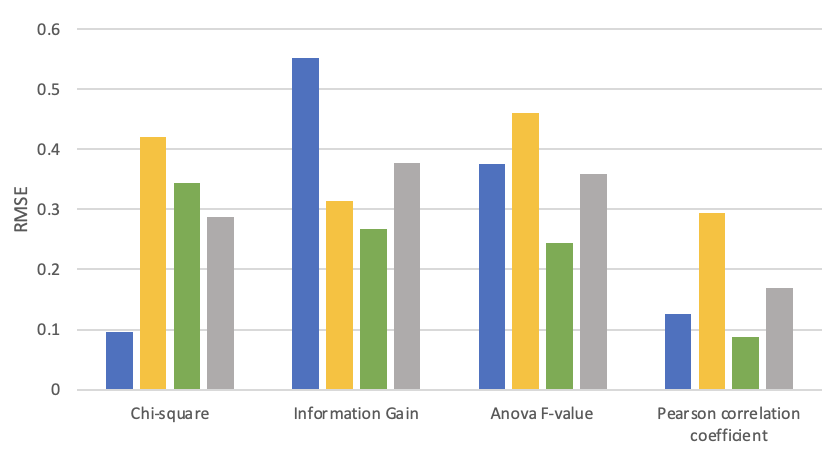
\includegraphics[width=6cm]{img/rq1figrmse.png} }}%
    \qquad
    \subfloat[\centering Kendall Tau distance of four feature selection techniques for datasets Adult (blue), Mushroom (yellow), Optic (green), and the average value of all datasets (grey)]{{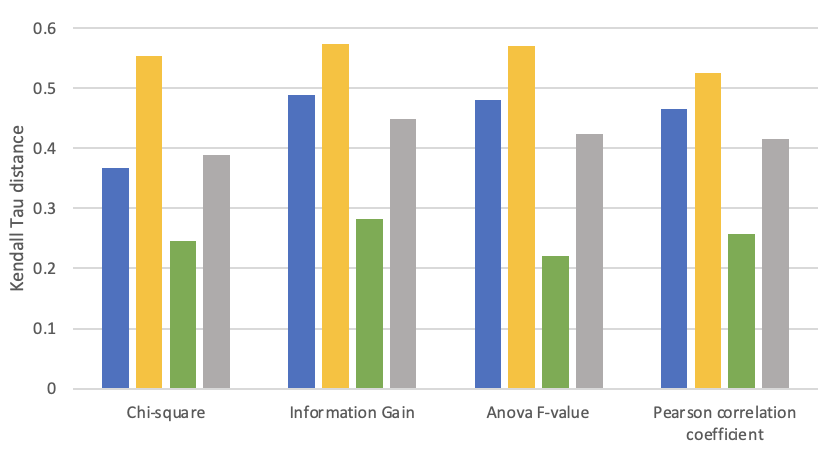
\includegraphics[width=6cm]{img/rq1figtaudist.png} }}%
    \caption{Heatmaps of Pearson correlation matrices for the Adult dataset.}
    \label{fig:selectionofselectiontech}
\end{figure}

\section{Features' correlation properties}
To gain insight into how the correlation between features is presered in anonymized datasets compared to the original dataset, we have depicted the heatmaps of feature's Pearson correlation scores in figures \ref{fig:heatmapsadult}, \ref{fig:heatmapsmushroom}, and \ref{fig:heatmapsoptic} for the Adult, Mushroom, and Optic datasets respectively. Only the first eleven relevant features are shown in the heatmap to improve visibility of the figure. The higher value (red) between two features shows that the associated features are more correlated, and the lower value (blue) shows less correlation. We observe that the scores in the correlation matrices for the differentially private datasets are a lot lower than in the original datasets. Therefore we include additional heatmaps with all self-correlations removed, this makes the heatmaps more visible because the range of the values in the heatmap is reduced.

From the heatmaps with self-correlations removed we can see that the correlation patterns have completely changed from the original dataset to the differentially private dataset. No correlation pattens from the original dataset could be identified in the differentially private dataset, meaning that values that were correlated before applying differential privacy are not correlated anymore after applying differential privacy.

\begin{figure}[H]
    \centering
    \subfloat[\centering Original Adult dataset]{{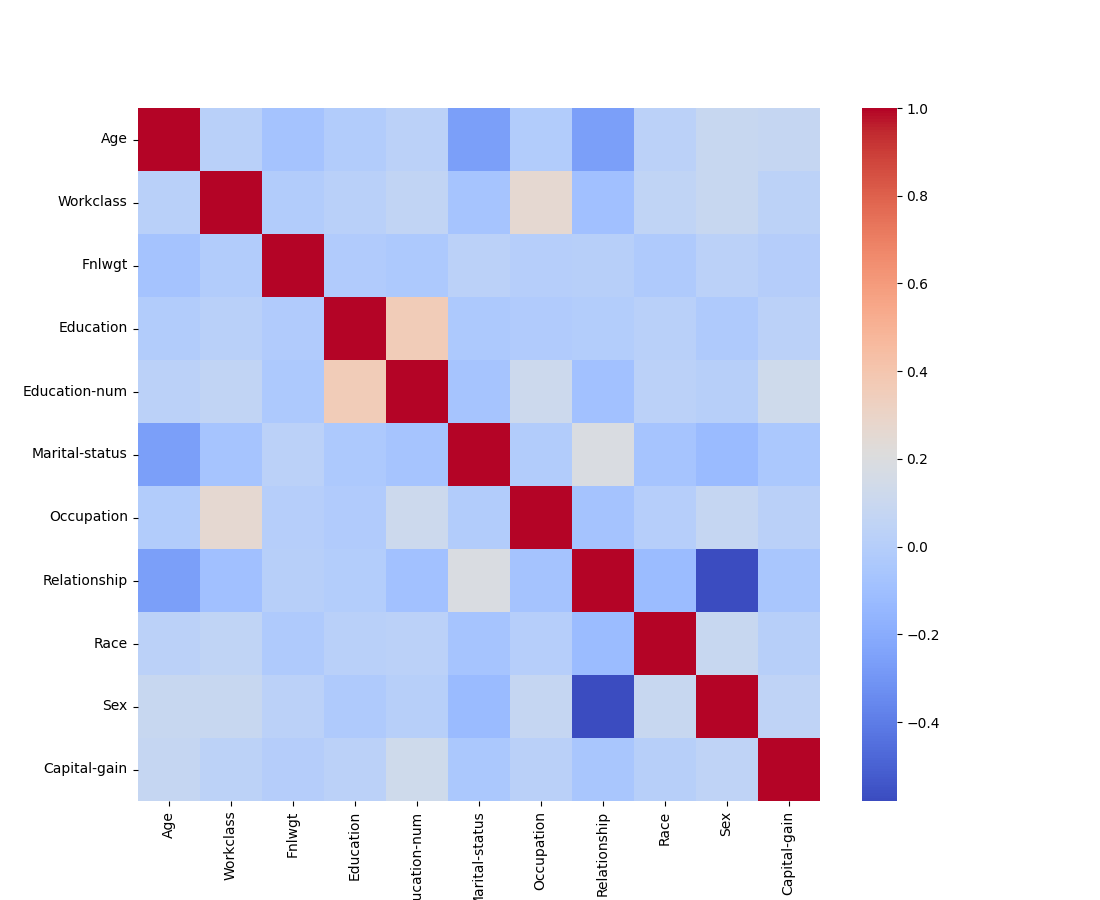
\includegraphics[width=4.7cm]{img/heatmapadultorig.png} }}%
    \qquad
    \subfloat[\centering Differentially private Adult dataset]{{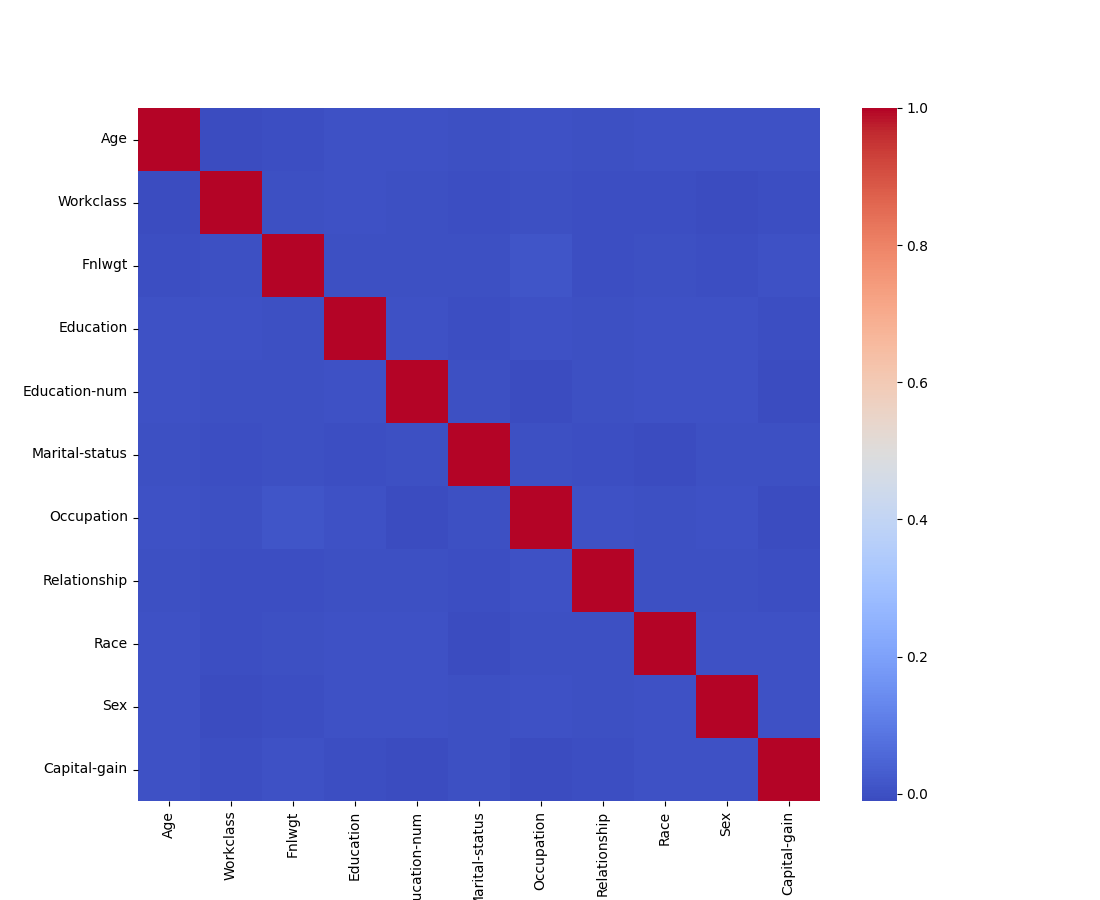
\includegraphics[width=4.7cm]{img/heatmapadultdp.png} }}%
    \qquad
    \subfloat[\centering Differentially private Adult dataset with self-correlation removed]{{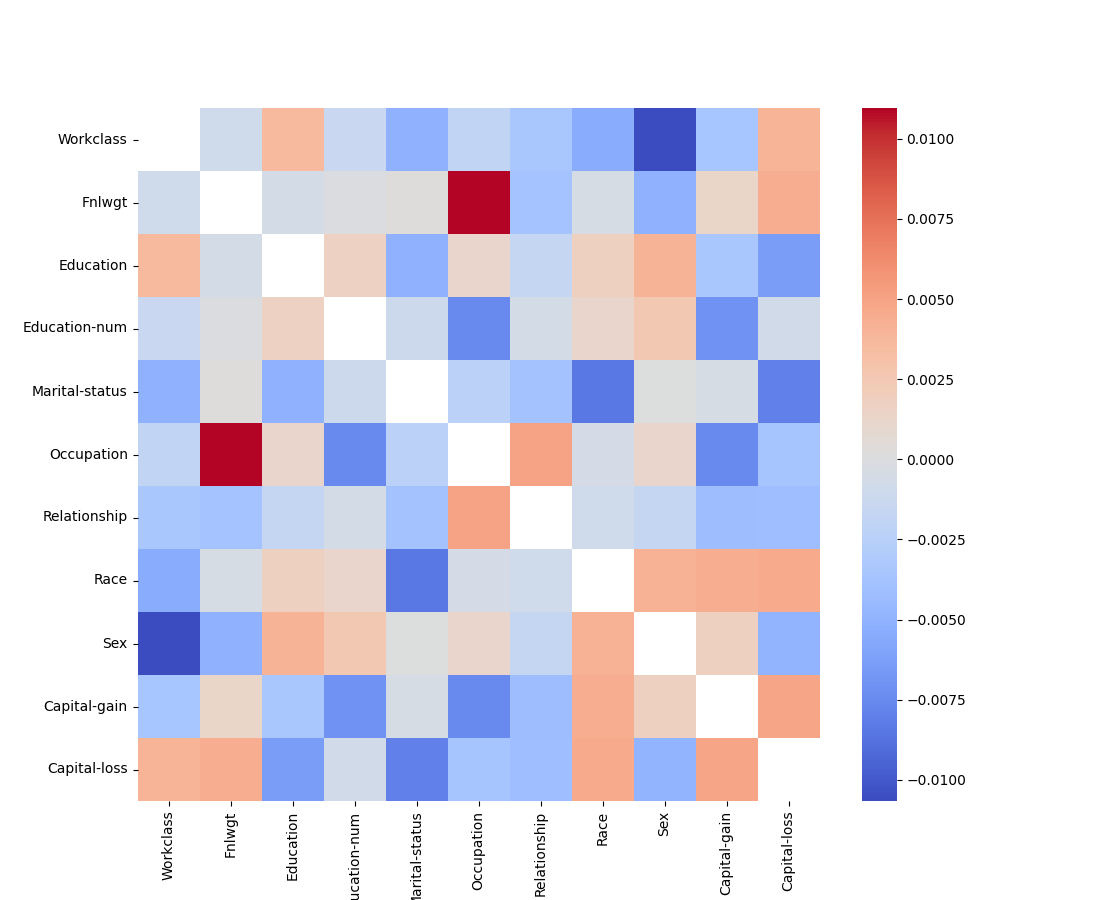
\includegraphics[width=4.7cm]{img/heatmapadultdp2.png} }}%
    \caption{Heatmaps of Pearson correlation matrices for the Adult dataset.}
    \label{fig:heatmapsadult}
\end{figure}

\begin{figure}[H]
    \centering
    \subfloat[\centering Original Mushroom dataset]{{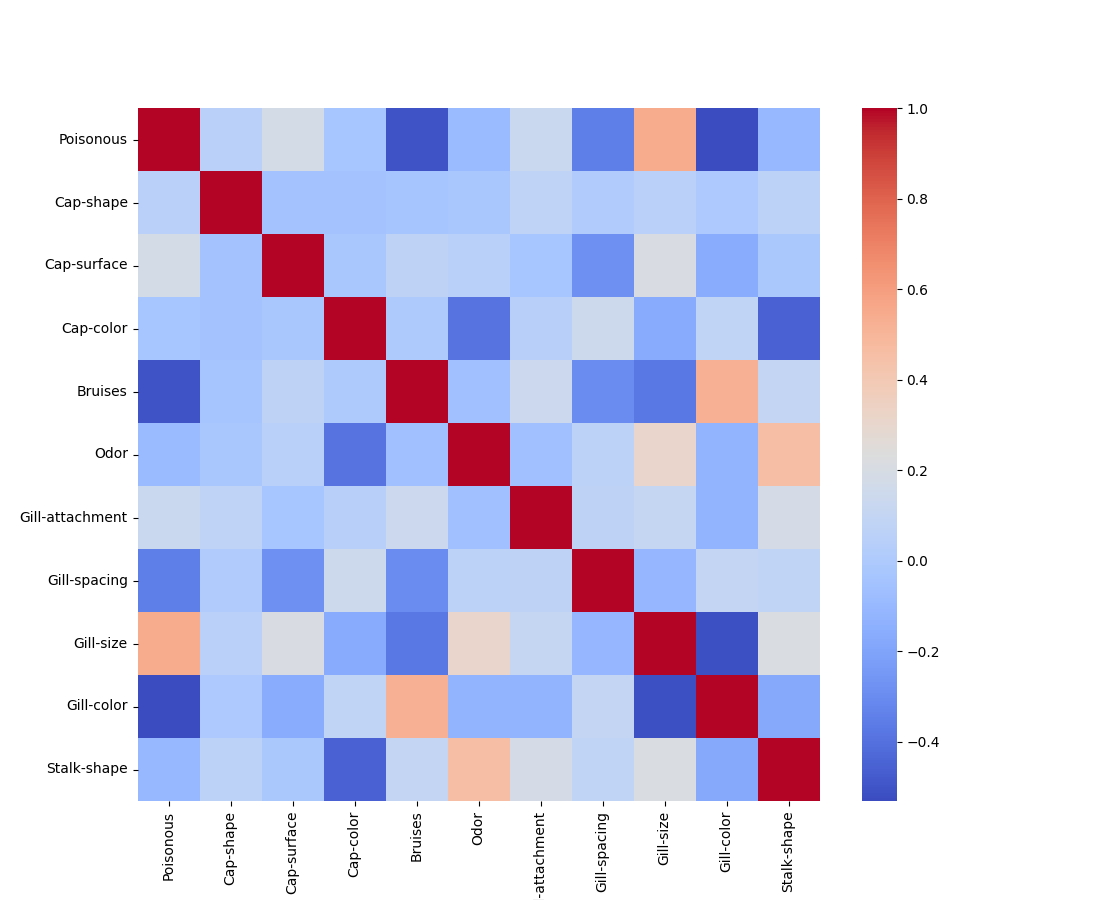
\includegraphics[width=4.7cm]{img/heatmapmushroomorig.png} }}%
    \qquad
    \subfloat[\centering Differentially private Mushroom dataset]{{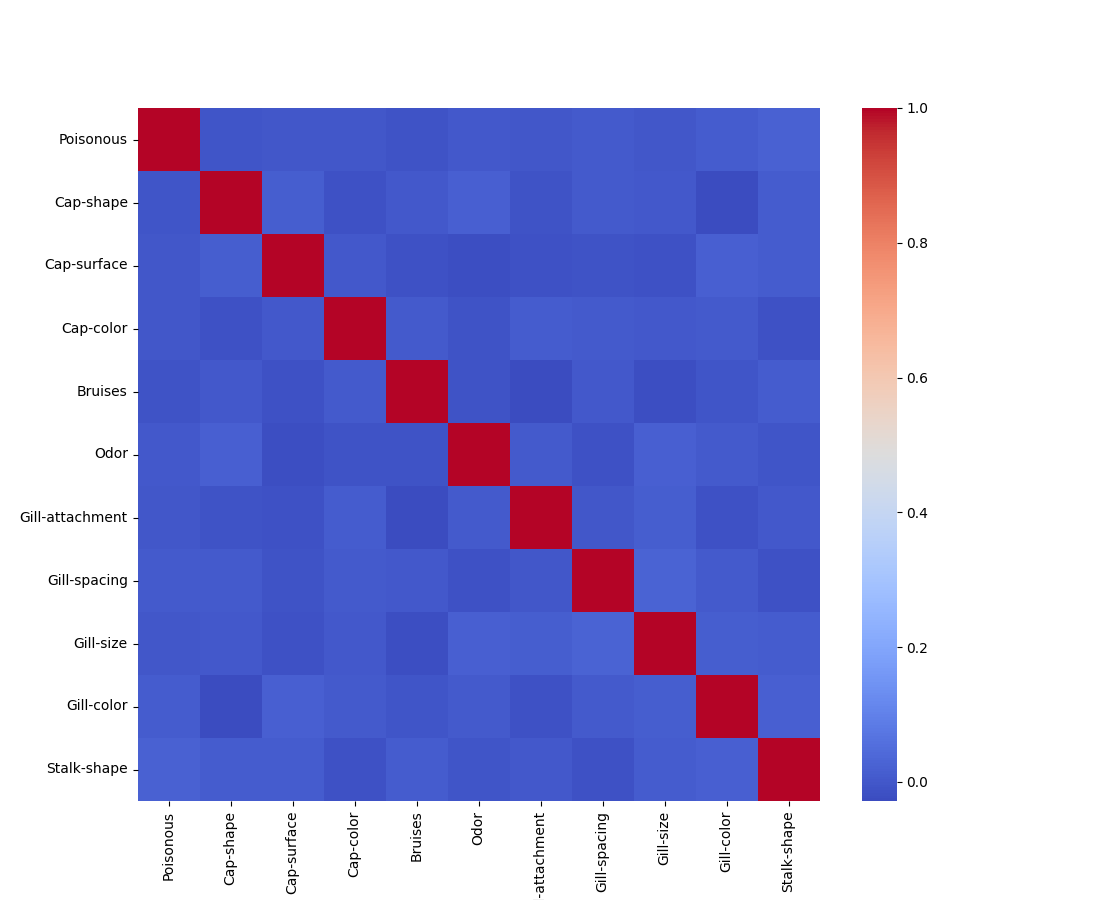
\includegraphics[width=4.7cm]{img/heatmapmushroomdp.png} }}%
    \qquad
    \subfloat[\centering Differentially private Mushroom dataset with self-correlation removed]{{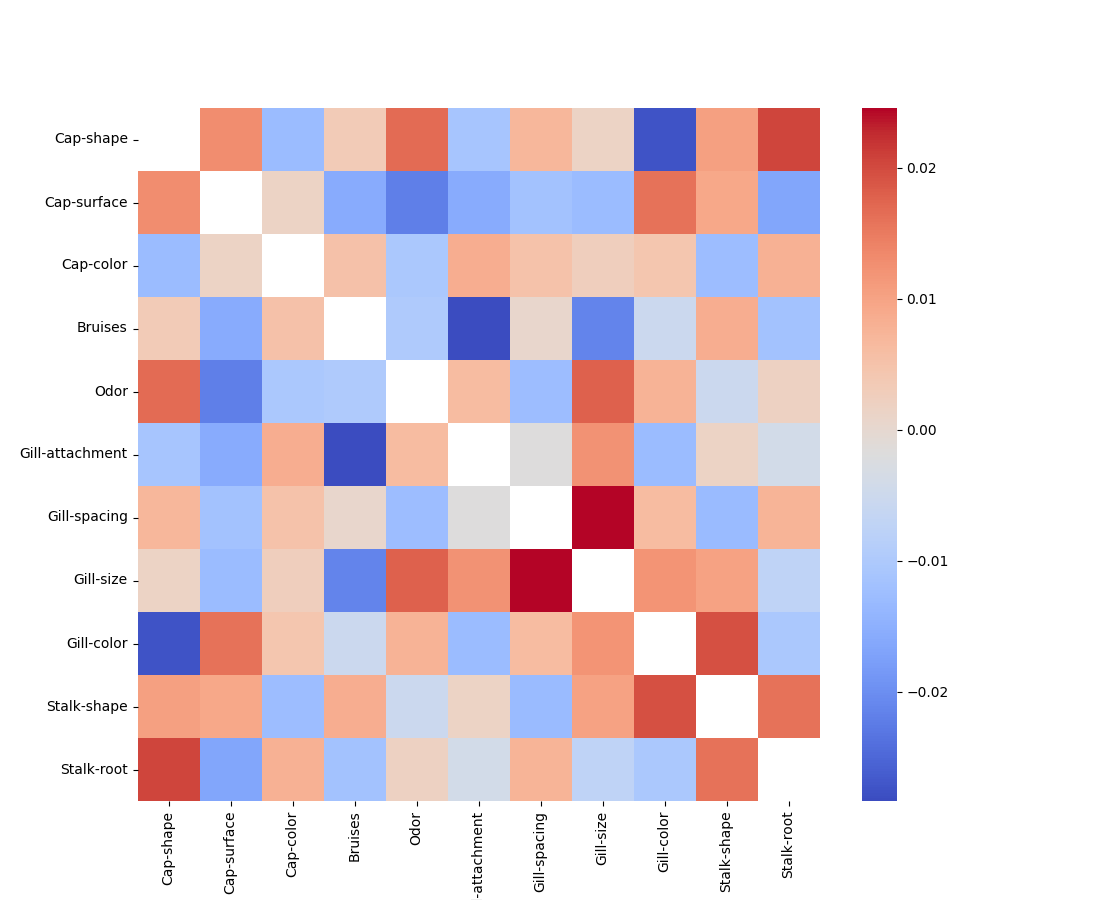
\includegraphics[width=4.7cm]{img/heatmapmushroomdp2.png} }}%
    \caption{Heatmaps of Pearson correlation matrices for the Mushroom dataset.}
    \label{fig:heatmapsmushroom}
\end{figure}

\begin{figure}[H]
    \centering
    \subfloat[\centering Original Optic dataset]{{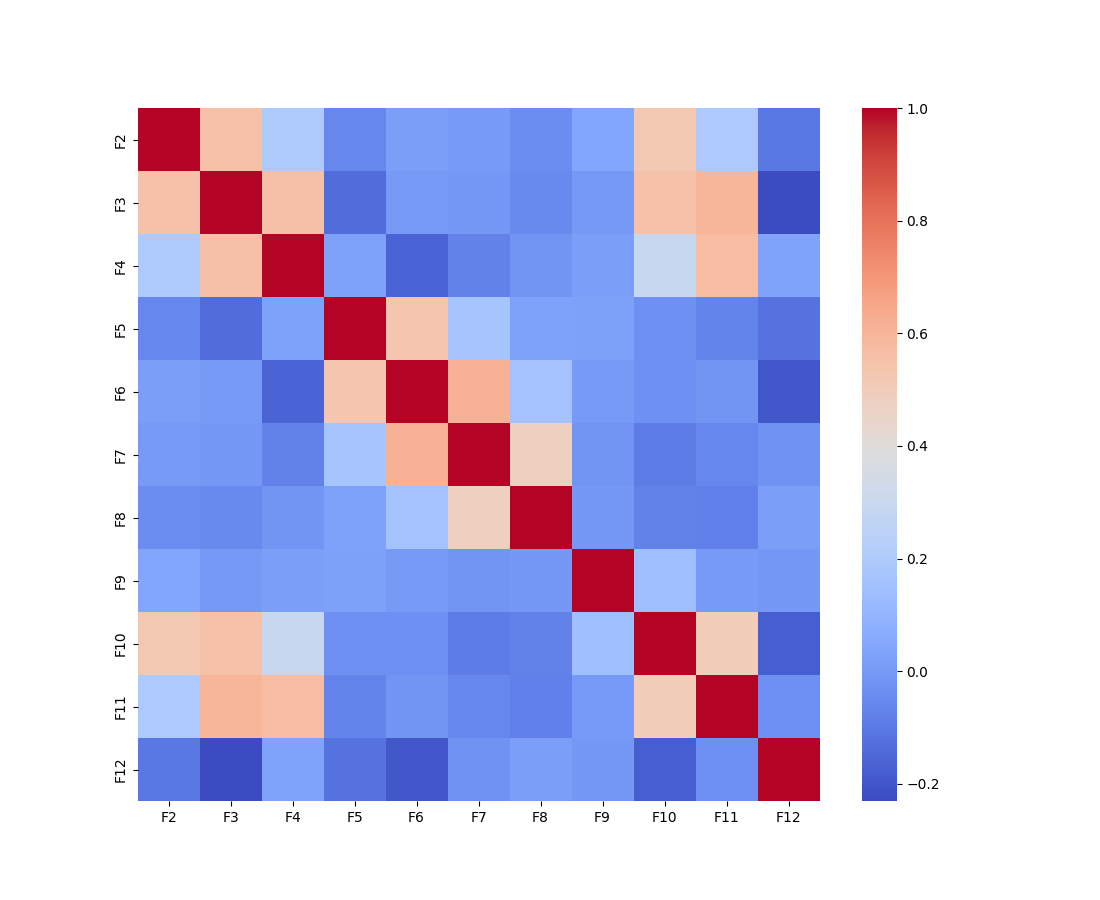
\includegraphics[width=4.7cm]{img/heatmapopticorig.png} }}%
    \qquad
    \subfloat[\centering Differentially private Optic dataset]{{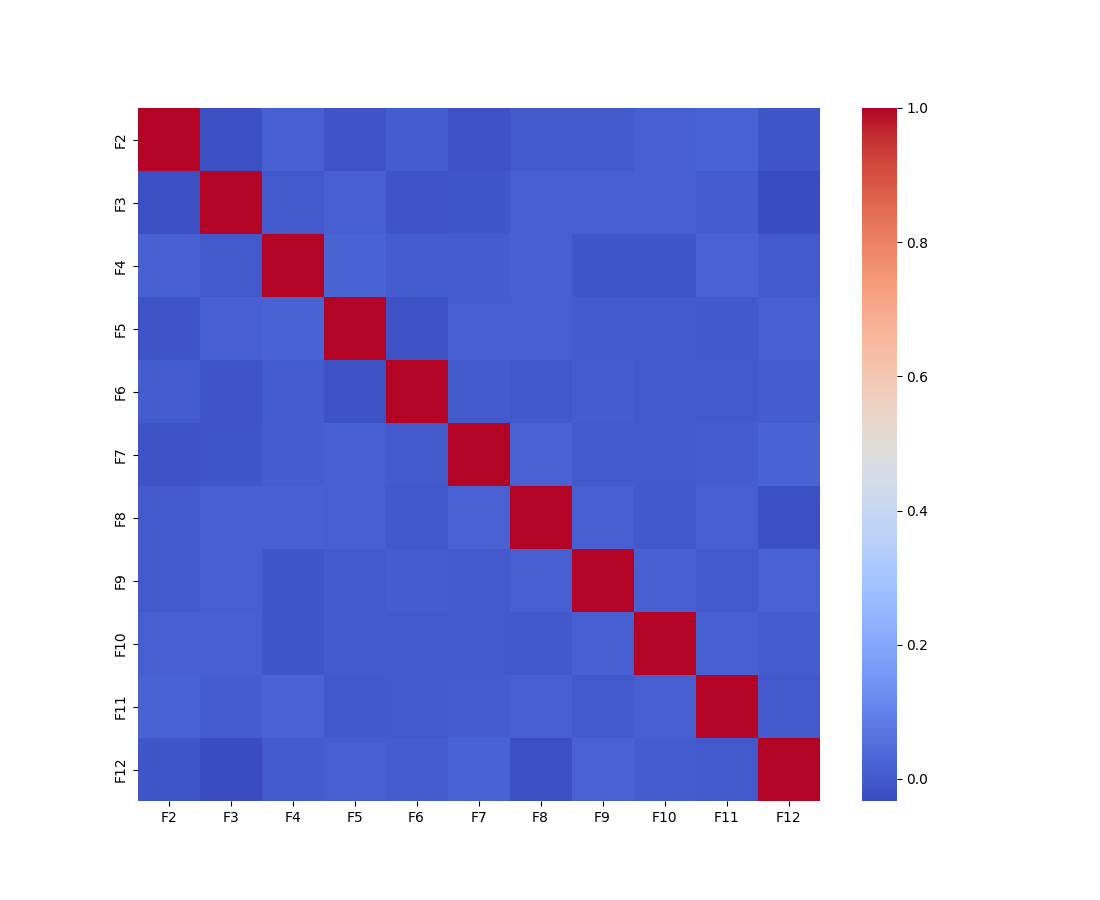
\includegraphics[width=4.7cm]{img/heatmapopticdp.png} }}%
    \qquad
    \subfloat[\centering Differentially private Optic dataset with self-correlation removed]{{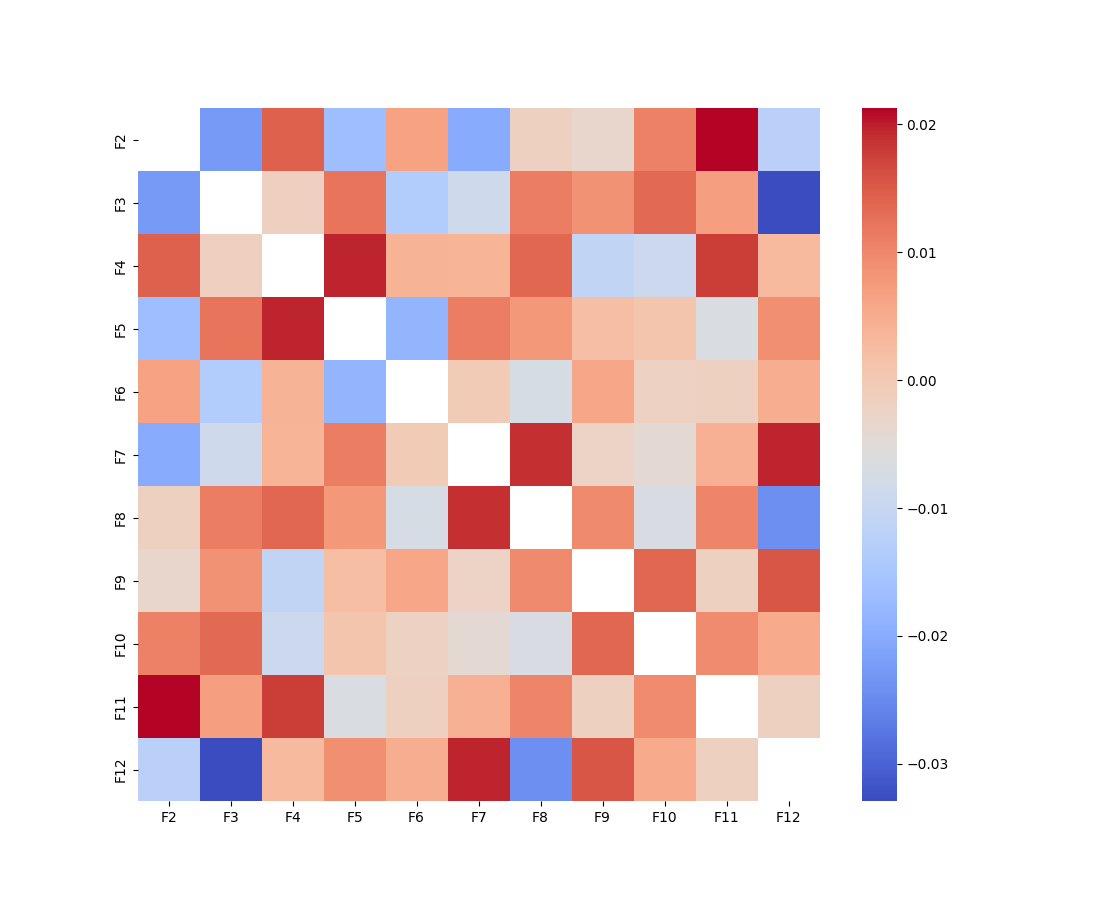
\includegraphics[width=4.7cm]{img/heatmapopticdp2.png} }}%
    \caption{Heatmaps of Pearson correlation matrices for the Optic dataset.}
    \label{fig:heatmapsoptic}
\end{figure}

\section{Impact of dataset properties}
The impact of dataset properties (dataset size, number of class labels, and number of features) on the RMSE between the Pearson correlation coefficient of the original dataset and the differentially private dataset is shown in figure \ref{fig:datasetparams}.

\begin{figure}[H]%
    \centering
    \subfloat[\centering Dataset size]{{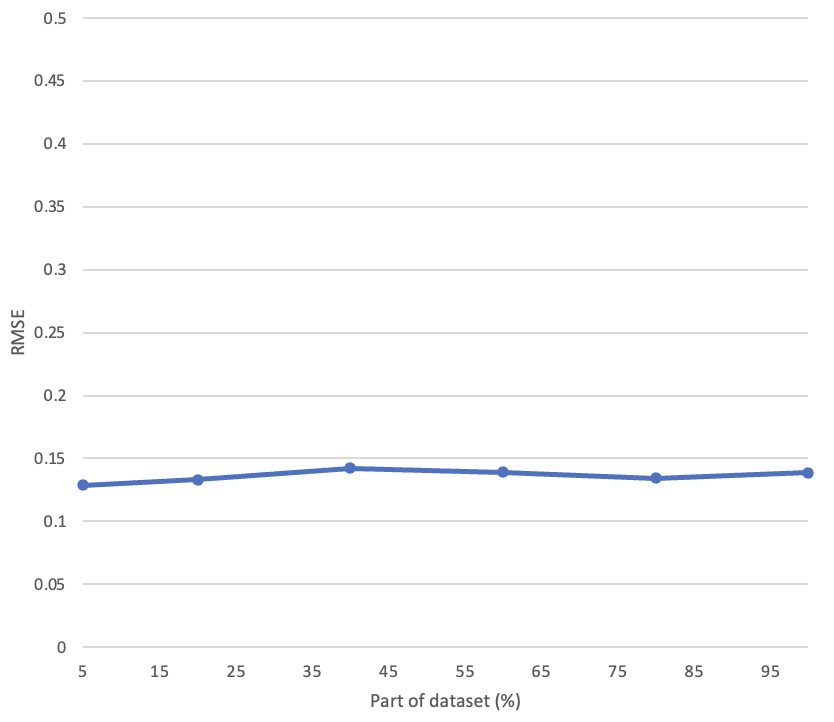
\includegraphics[width=4.5cm]{img/datasetsize.png} }}%
    \qquad
    \subfloat[\centering Number of class labels]{{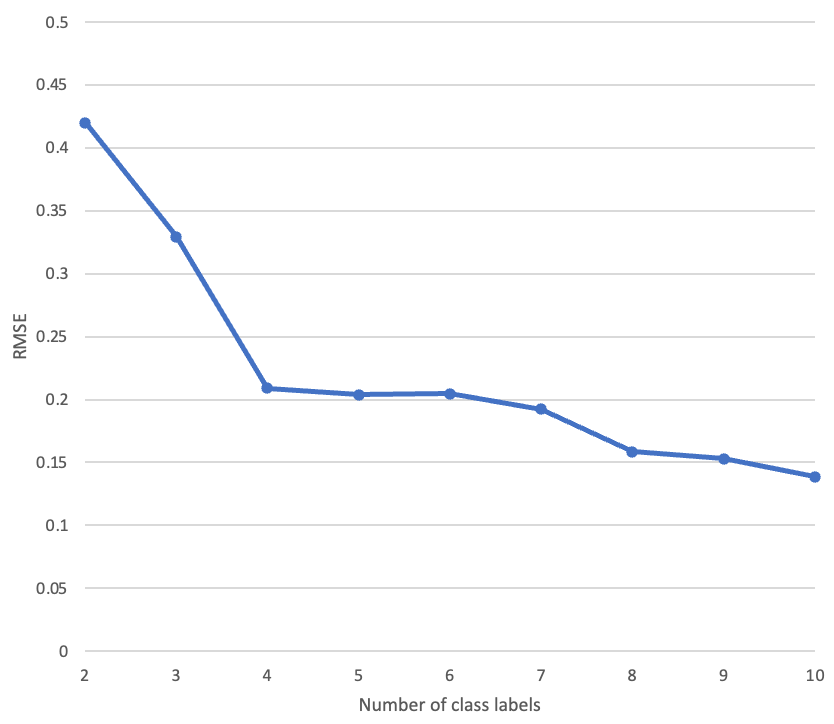
\includegraphics[width=4.5cm]{img/classlabels.png} }}%
    \qquad
    \subfloat[\centering Number of features]{{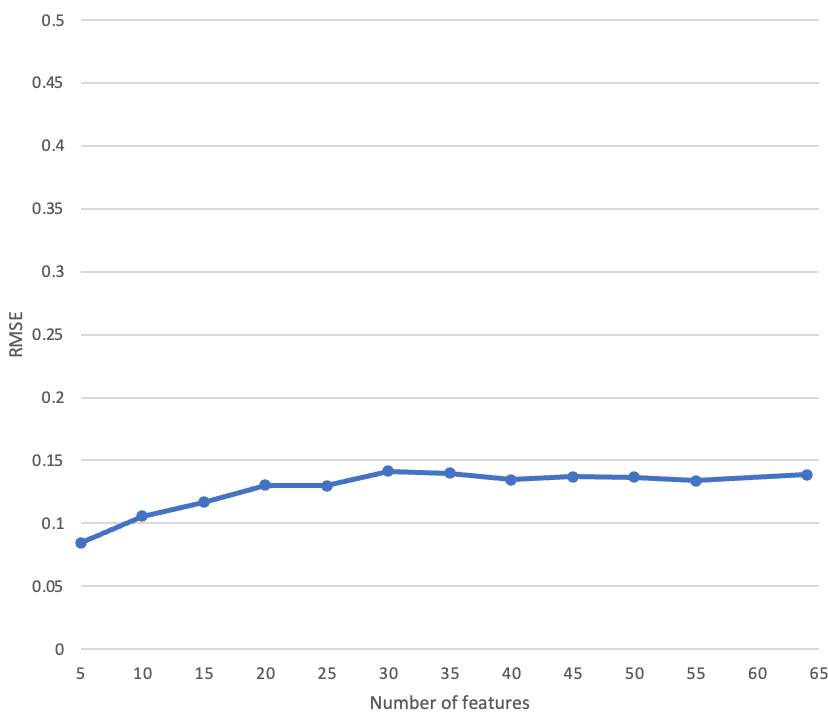
\includegraphics[width=4.5cm]{img/features.png} }}%
    \caption{The impact of varying the dataset parameters on the RMSE between the Pearson correlation coefficient of the original dataset and the differentially private dataset.}%
    \label{fig:datasetparams}%
\end{figure}

We observe that the dataset size does not have much impact on the Pearson correlation coefficient after applying differential privacy. 

However, the number of class labels has a large impact on the Pearson correlation coefficient. When the number of class labels is smaller than 4, the Pearson correlation coefficient is going down for larger numbers of class labels. From more than 4 class labels the Pearson correlation coefficient stabilizes and slightly goes down again for number of class labels higher than 6.

The number of features only affects the Pearson correlation coefficient for 30 features or less, but only slightly. With a number of features below 30 the RMSE between Pearson correlations is better than for 30 or more features. For 30 or more features the Pearson correlation coefficient is stable.\\

All observed Pearson correlation values for varying dataset parameters are within an acceptable range, except for the number of class labels below 4.

\section{Impact of differential privacy parameter}
The impact of the differential privacy parameter ($\epsilon$) on the RMSE between the Pearson correlation coefficient of the original dataset and the differentially private dataset is shown in figure \ref{fig:datasetparams}.

\begin{figure}[H]
    \centering
    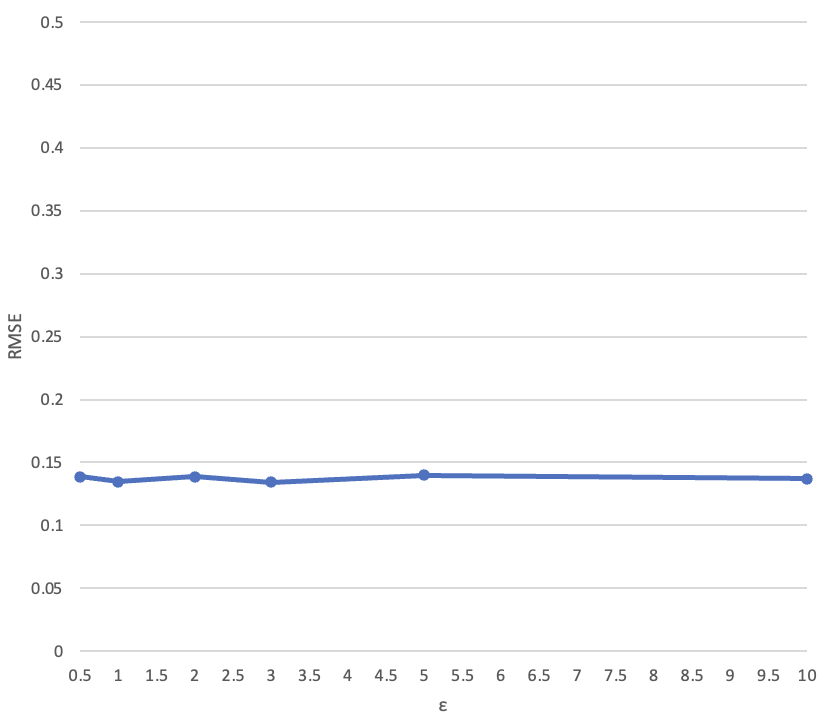
\includegraphics[width=5cm]{img/epsilon.png}
    \caption{The impact of varying the differential privacy parameter $\epsilon$ on the RMSE between the Pearson correlation coefficient of the original dataset and the differentially private dataset.}
    \label{fig:epsilonparam}
\end{figure}

The value of $\epsilon$ has no noticable effect on the Pearson correlation coefficient after applying differential privacy, its value is stable for all $\epsilon$ values. The value of $\epsilon$ might however influence other statistics that are beyond this research.

\section{Trained classifiers' impact}
Table 4.1 shows the classifier accuracy for Naive Bayes (NB), Decision Tree (DT), k-Nearest Neighbors (kNN), Random Forest (RF), Linear Regression (LR), and AdaBoost (AB) after keeping 20\% of the most relevant using Pearson correlation in original and differentially private datasets. The difference is shown in the last column.

All classifiers show similar differences and are positive close to 0, meaning that the performance of all classifiers is slightly worse when using the differentially private dataset than when using the original dataset. This small difference can be because of the small number of class labels in the Adult dataset.

\begin{table}[H]
\label{fig:classifiers}
\centering
\begin{tabular}{lllll}
Dataset                & Classifier & Original & Differentially private & diff. \\ \hline
\multirow{6}{*}{Adult} & NB         & 0.781    & 0.727                  & 0.054 \\
                       & DT         & 0.775    & 0.757                  & 0.018 \\
                       & kNN        & 0.771    & 0.724                  & 0.047 \\
                       & RF         & 0.769    & 0.747                  & 0.022 \\
                       & LR         & 0.781    & 0.755                  & 0.026 \\
                       & AB         & 0.784    & 0.749                  & 0.035 \\ \cline{2-5} 
                       & avg.       & 0.778    & 0.744                  & 0.034
\end{tabular}
\caption{Classifiers' accuracy for Naive Bayes (NB), Decision Tree (DT), k-Nearest Neighbors (kNN), Random Forest (RF), Linear Regression (LR), and AdaBoost (AB) after keeping 20\% of the most relevant using Pearson correlation in original and differentially private datasets.}
\end{table}


% \input{sections/discussion}
% \input{sections/related_work}
% \chapter{Conclusion}
\label{ch:conclusion}

From our first research question we conclude that the Pearson correlation coefficient is the best method for preserving the scores of features in differentially private datasets in comparison to the original dataset. The comparison of feature scores between the original dataset and the differentially private dataset can best be done by calculating the Root Mean Square Error.\\

From the created Pearson correlation matrix heatmaps we observed that correlation patterns between features in a dataset completely change when applying differential privacy.\\

The only noteworthy parameter that influences the Pearson correlation coefficient is the number of class labels, when the number of class labels is below 4 the difference in Pearson correlation coefficient is far worse than when the number of class labels is larger than four.
The number of features slightly influences the Pearson correlation scores, with number of features below 30 difference in Pearson correlation scores is better than with number of features above 30.\\

The differential privacy parameter $\epsilon$ does not cause a change in Pearson correlation scores at all, for all tested $\epsilon$ values the RMSE between correlation scores before and after applying differential privacy remained the same. \\

From the classifier analysis we observed a slightly worse classifier score when classifiers were trained on a differentially private dataset, compared to the equivalent original dataset. All different classifiers showed similar results.

\section{Future work}
After answering our research question there is some future work left. 

An in-depth analysis can be done on why the Pearson correlation matrices change so much after differential privacy is applied to a dataset. The change in dataset parameters and differentially privacy parameter can be investigated for other datasets than only the Optic dataset, and the classifier analysis can be done on other datasets.

Also, an analysis and comparison can be done when using another differential privacy framework than PrivSyn.\\

A future study can be done in comparing the results of this research to the results of Feature Selection on Anonymized Datasets \cite{originalpaper}. Then a conclusion can be made on the differences in effects of feature selection on anonymized datasets and feature selection on differentially private datasets.
% \input{sections/acknowledgements}

\printbibliography[heading=bibintoc]
\printglossaries%

% \input{sections/appendix}

%comment out in the final version
%\listoftodos[Notes]

\end{document}
